\documentclass{article}
\usepackage[margin=1in]{geometry}
\usepackage{amsmath,amsthm,amssymb}
\usepackage{bbm,enumerate,mathtools}
\usepackage{tikz,pgfplots}
\usepackage{chessboard}
\usepackage[hidelinks]{hyperref}
\usepackage{multicol} % Problem 35

\newenvironment{question}{\begin{trivlist}\item[\textbf{Question.}]}{\end{trivlist}}
\newenvironment{note}{\begin{trivlist}\item[\textbf{Note.}]}{\end{trivlist}}
\newenvironment{references}{\begin{trivlist}\item[\textbf{References.}]}{\end{trivlist}}
\newenvironment{related}{\begin{trivlist}\item[\textbf{Related.}]\end{trivlist}\begin{enumerate}}{\end{enumerate}}


\begin{document}
\rating{3}{2}
Consider ways of partitioning nonattacking rooks in such a way that no rook lies
in the convex hull of its partition. Let $a(\sigma)$ be the minimum number of parts
of such a partition.
\begin{figure}[ht!]
  \centering
  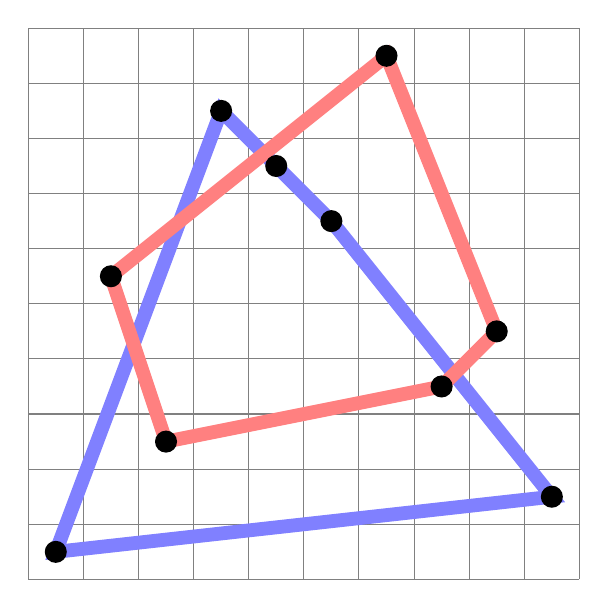
\begin{tikzpicture}[scale=0.7]
    \draw[gray] (0,0) grid (10,10);
    \draw[blue!50, line width=5] (0.5,0.5)--(3.5,8.5)--(4.5,7.5)--(5.5,6.5)--(9.5,1.5)--cycle;
    \draw[red!50, line width=5] (1.5,5.5)--(2.5,2.5)--(7.5,3.5)--(8.5,4.5)--(6.5,9.5)--cycle;
    \foreach \x/\y in {1/0, 2/5, 3/2, 4/8, 5/7, 6/6, 7/9, 8/3, 9/4, 10/1} {
      \fill (\x - 0.5, \y + 0.5) circle (0.2);
    }
  \end{tikzpicture}
  \caption{
    An illustration showing that $a(\sigma) = 2$ for $\sigma = 16398710452 \in S_{10}$.
  }
\end{figure}

\begin{question}
  What is the expected value of $a(\sigma)$ for a uniformly random $\sigma \in S_n$?
\end{question}

\begin{related}
  \item What if each point must be on the corner of the convex hull?
  \item What is the maximum number of convex hulls required?
  \item What is the expected number of convex hulls?
  (i.e. how many different ways can a $\sigma$ be partitioned into
  $a(\sigma)$ convex hulls?
  \item What if the convex hulls are not allowed to overlap?
  \item What is the expected value of the largest subset of
    $((1, \sigma(1)), \hdots, (n, \sigma(n)))$ such that no points are in the
    interior of the convex hull?
  \item What if this is done for non-attacking queens?
  \item What if this is done for an arbitrary configuration of $k$ pieces on an
    $n \times m$ board?
  \item What if the convex hull of the permutation is taken, and then the convex
  hull of the interior, and the convex hull of that interior and so on?
  \item What if a no three-on-a-line rule is used instead?
  No $k+2$ on a degree $k$ polynomial?
\end{related}

\begin{note}
  \item $A156831(n) = \{ \sigma \in S_n : a(\sigma) = 1 \}$.
\end{note}

\begin{references}
  \item \url{https://oeis.org/A156831}
  \item Problem 6, 7, 8.
\end{references}

\end{document}
